\documentclass[12pt,a4paper]{article}

% Packages
\usepackage{geometry}
\geometry{margin=1in}
\usepackage{fancyhdr}
\usepackage{titlesec}
\usepackage{listings}
\usepackage{xcolor}
\usepackage{graphicx} 

% Header & Footer
\pagestyle{fancy}
\fancyhf{}
\rhead{C++ - Assignment 1}
\lhead{Kamithkar Vinod}
\cfoot{\thepage}

% Title formatting
\titleformat{\section}{\large\bfseries}{Problem \thesection:}{0.5em}{}
\titleformat{\subsection}[runin]{\bfseries}{Code:}{0.5em}{}[---]
\titleformat{\subsubsection}[runin]{\bfseries}{Output:}{0.5em}{}[---]

% Code style
\lstset{
    language=cpp,
    basicstyle=\ttfamily\small,
    keywordstyle=\color{blue}\bfseries,
    commentstyle=\color{gray}\itshape,
    stringstyle=\color{red},
    showstringspaces=false,
    numbers=left,
    numberstyle=\tiny\color{gray},
    frame=single,
    breaklines=true
}

% Document Start
\begin{document}

% Title Page
\begin{center}
    \LARGE \textbf{Assignment - 1} \\[0.5cm]
    \Large \textbf{C++} \\[1cm]

    \begin{tabular}{rl}
        \textbf{Name:} & Kamithkar Vinod \\
        \textbf{Course:} & PG DAC AUGUST 2025 \\
        \textbf{PRN:} & 250850320040 \\
        \textbf{Form No:} & 250500480 \\
        \textbf{Date:} & 07-10-2025 \\
    \end{tabular}
\end{center}

\vspace{1cm}
\hrule
\vspace{0.5cm}

% Problems
% 1
\section{}
\textbf{Task:} Write a C++ program that prints "Hello, World!" to the console.

\subsection{}
\begin{lstlisting}
#include <iostream>
using namespace std;

int main() {
    cout << "Hello, World!" << endl;
    return 0;
}
\end{lstlisting}

\subsubsection{1}
\begin{center}
    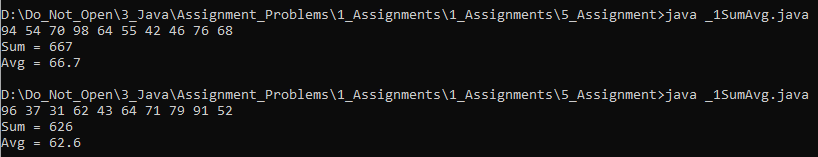
\includegraphics[width=0.8\textwidth]{1.png}
\end{center}


% 2

\section{}
\textbf{Task:} Write a C++ program that takes two integer inputs from the user and prints their sum.
\subsection{}
\begin{lstlisting}
#include <iostream>
using namespace std;

int main() {
    int num1, num2, sum;

    cout << "Enter first integer: ";
    cin >> num1;

    cout << "Enter second integer: ";
    cin >> num2;

    sum = num1 + num2;

    cout << "The sum of " << num1 << " and " << num2 << " is: " << sum << endl;

    return 0;
}
\end{lstlisting}

\subsubsection{}
\begin{center}
    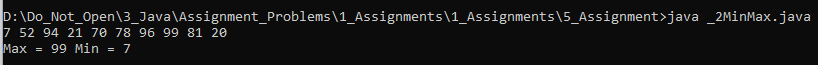
\includegraphics[width=0.8\textwidth]{2.png}
\end{center}

% 3

\section{}
\textbf{Task:} Write a C++ program to swap two numbers without using a third variable

\subsection{}
\begin{lstlisting}
#include <iostream>
using namespace std;

int main() {
    int a, b;

    cout << "Enter two numbers: ";
    cin >> a >> b;

    cout << "\nBefore swapping: a = " << a << ", b = " << b << endl;

    // Method 1: Using arithmetic operations
    a = a + b;
    b = a - b;
    a = a - b;

    // Alternative Method 2: Using bitwise XOR (uncomment to test)
    // a = a ^ b;
    // b = a ^ b;
    // a = a ^ b;

    cout << "After swapping: a = " << a << ", b = " << b << endl;

    return 0;
}

\end{lstlisting}

\subsubsection{}
\begin{center}
    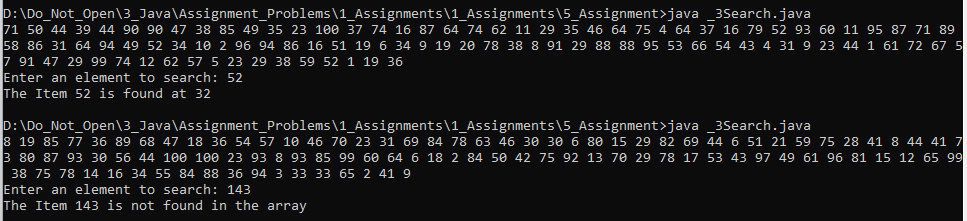
\includegraphics[width=0.8\textwidth]{3.png}
\end{center}

% 4

\section{}
\textbf{Task:} Write a C++ program that checks whether a number entered by the user is even or odd.

\subsection{}
\begin{lstlisting}
#include <iostream>
using namespace std;

bool is_even(int n) {
    return n % 2 == 0;
}

int main() {
    int n;
    cout << "Enter a number: ";
    cin >> n;
    
    if (is_even(n)) {
        cout << n << " is even." << endl;
    } else {
        cout << n << " is odd." << endl;
    }
    
    return 0;
}
\end{lstlisting}

\subsubsection{}
\begin{center}
    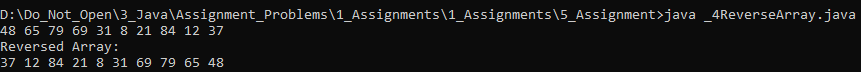
\includegraphics[width=0.8\textwidth]{4.png}
\end{center}

% 5

\section{}
\textbf{Task:} Write a C++ program that takes two numbers and an operator (+, -, *, /) as input and performs the corresponding operation.

\subsection{}
\begin{lstlisting}
#include <iostream>
using namespace std;

int main() {
    double num1, num2;
    char op;

    cout << "Enter first number: ";
    cin >> num1;

    cout << "Enter an operator (+, -, *, /): ";
    cin >> op;

    cout << "Enter second number: ";
    cin >> num2;

    double result;

    switch (op) {
        case '+':
            result = num1 + num2;
            cout << "Result: " << num1 << " + " << num2 << " = " << result << endl;
            break;
        case '-':
            result = num1 - num2;
            cout << "Result: " << num1 << " - " << num2 << " = " << result << endl;
            break;
        case '*':
            result = num1 * num2;
            cout << "Result: " << num1 << " * " << num2 << " = " << result << endl;
            break;
        case '/':
            if (num2 != 0) {
                result = num1 / num2;
                cout << "Result: " << num1 << " / " << num2 << " = " << result << endl;
            } else {
                cout << "Error: Division by zero is not allowed!" << endl;
            }
            break;
        default:
            cout << "Invalid operator! Please use +, -, *, or /." << endl;
            break;
    }

    return 0;
}

\end{lstlisting}

\subsubsection{}
\begin{center}
    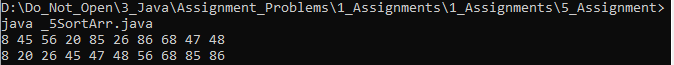
\includegraphics[width=0.8\textwidth]{5.png}
\end{center}

% 6

\section{}
\textbf{Task:} Write a C++ program that takes n numbers as input, stores them in an array, and finds the largest number.

\subsection{}
\begin{lstlisting}
#include <iostream>
#include <cstdlib>  // For rand() and srand()
#include <ctime>    // For time()
using namespace std;

int main() {
    int n;

    cout << "Enter the number of elements: ";
    cin >> n;

    if (n <= 0) {
        cout << "Invalid input! Number of elements must be greater than zero." << endl;
        return 1;
    }

    int arr[n];

    // Seed the random number generator
    srand(time(0));

    cout << "\nGenerated random numbers:\n";
    for (int i = 0; i < n; i++) {
        arr[i] = rand() % 100; // random values between 0 and 99
        cout << arr[i] << " ";
    }
    cout << endl;

    int largest = arr[0];

    for (int i = 1; i < n; i++) {
        if (arr[i] > largest) {
            largest = arr[i];
        }
    }

    cout << "\nThe largest number is: " << largest << endl;

    return 0;
}

\end{lstlisting}

\subsubsection{}
\begin{center}
    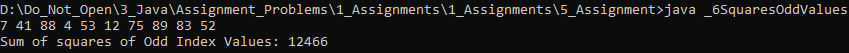
\includegraphics[width=0.8\textwidth]{6.png}
\end{center}

% 7

\section{}
\textbf{Task:} Write a C++ program that takes an integer input and calculates the sum of its digits.

\subsection{}
\begin{lstlisting}
#include <iostream>
using namespace std;

int main() {
    int n;
    cout << "Enter a Number: ";
    cin >> n;
    int sum = 0;
    while (n > 0) {
        sum += n % 10;
        n /= 10;
    }
    cout << "Sum of digits: " << sum << endl;
    return 0;
}
\end{lstlisting}

\subsubsection{}
\begin{center}
    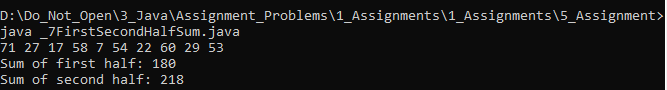
\includegraphics[width=0.8\textwidth]{7.png}
\end{center}

% 8

\section{}
\textbf{Task:} Write a C++ program to take n elements in an array and print them in reverse order.

\subsection{}
\begin{lstlisting}
#include <iostream>
using namespace std;

/**
 * Reverses the elements of an array in place.
 *
 * @param arr The array to reverse.
 * @param n The number of elements in the array.
 */
void reverse_array(int arr[], int n) {
    int start = 0;
    int end = n-1;
    while (start < end) {
        int temp = arr[start];
        arr[start] = arr[end];
        arr[end] = temp;
        start++;
        end--;
    }
}


/**
 * Example program that demonstrates the use of the reverse_array function.
 */
int main() {
    int arr[] = {1, 2, 3, 4, 5};
    int n = sizeof(arr) / sizeof(arr[0]);

    // Reverse the array in place
    reverse_array(arr, n);

    // Print the reversed array
    for (int i = 0; i < n; i++) {
        cout << arr[i] << " ";
    }
    cout << endl;

    return 0;
}
\end{lstlisting}

\subsubsection{}
\begin{center}
    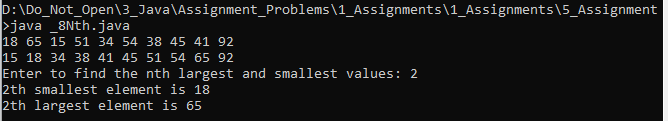
\includegraphics[width=0.8\textwidth]{8.png}
\end{center}

% 9

\section{}
\textbf{Task:} Write a C++ program to check if a given number is palindromic (reads the same forward and backward).

\subsection{}
\begin{lstlisting}
#include <iostream>
using namespace std;

/**
 * Checks if a given number is a palindrome.
 *
 * @param n The number to check.
 * @return true if the number is a palindrome, false otherwise.
 */ 
bool is_palindrome_number(int n) {  
    int reversed = 0;
    int original = n;
    
    while (n > 0) {
        int digit = n % 10;
        reversed = reversed * 10 + digit;
        n /= 10;
    }
    
    return original == reversed;
}

/**
 * Example program that demonstrates the use of the is_palindrome_number function.
 */
int main() {
    int n;
    cout << "Enter a number: ";
    cin >> n;
    
    if (is_palindrome_number(n)) {
        cout << n << " is a palindrome number." << endl;
    } else {
        cout << n << " is not a palindrome number." << endl;
    }
    
    return 0;
}

/**
 * Checks if a given number is a palindrome.
 *
 * A palindrome is a number that reads the same backwards as forwards.
 *
 * @param n The number to check.
 * @return true if the number is a palindrome, false otherwise.
 */

\end{lstlisting}

\subsubsection{}
\begin{center}
    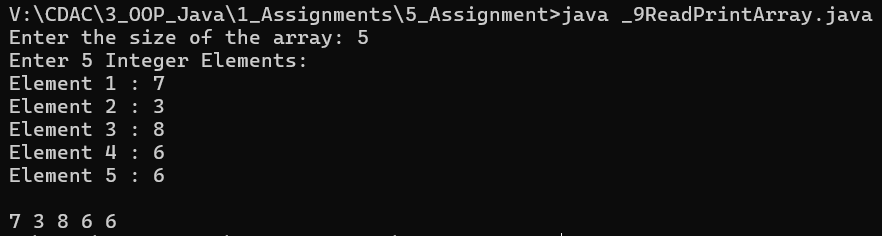
\includegraphics[width=0.8\textwidth]{9.png}
\end{center}

% 10

\section{}
\textbf{Task:} Write a C++ program to print the Fibonacci series up to n terms.

\subsection{}
\begin{lstlisting}
#include <iostream>
using namespace std;
/**
 * Prints the first n terms of the Fibonacci series.
 *
 * The Fibonacci series is a sequence of numbers in which each number is the sum of the two preceding numbers.
 *
 * @param n The number of terms to print.
 */
void print_fibonacci_series(int n) {
    int a = 0, b = 1, c;
    if (n == 0) return;
    cout << a << " ";
    if (n == 1) return;
    cout << b << " ";
    for (int i = 2; i < n; i++) {
        c = a + b;
        cout << c << " ";
        a = b;
        b = c;
    }
}

/**
 * The main function of the program.
 *
 * Prompts the user to enter a number, then uses that number to print the first n terms of the Fibonacci series.
 *
 * @return 0 if the program runs successfully.
 */
int main() {
    int n;
    cout << "Enter the number of terms: ";
    cin >> n;

    // Print the first n terms of the Fibonacci series
    print_fibonacci_series(n);

    return 0;
}

\end{lstlisting}

\subsubsection{}
\begin{center}
    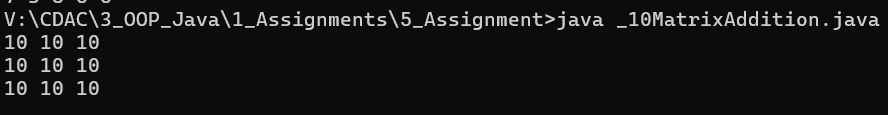
\includegraphics[width=0.8\textwidth]{10.png}
\end{center}

% 11

\section{}
\textbf{Task:} Write a C++ program that takes a string as input and counts the number of vowels (a, e, i, o, u).

\subsection{}
\begin{lstlisting}
#include <string>
#include <iostream>
using namespace std;
/**
 * Counts the number of vowels in a given string.
 *
 * @param str The string to count the vowels from.
 * @return The number of vowels in the string.
 */
int count_vowels(const string& str) {
    int count = 0;
    for (char c : str) {
        switch (c) {
            case 'a':
            case 'e':
            case 'i':
            case 'o':
            case 'u':
                count++;
                break;
            default:
                break;
        }
    }
    return count;
}

/**
 * The main function of the program.
 *
 * Prompts the user to enter a string, then uses the count_vowels function to count the number of vowels in the string.
 *
 * @return 0 if the program runs successfully.
 */
int main() {
    string str;
    cout << "Enter a string: ";
    cin >> str;
    int count = count_vowels(str);
    cout << "Number of vowels: " << count << endl;
    return 0;
}

\end{lstlisting}

\subsubsection{}
\begin{center}
    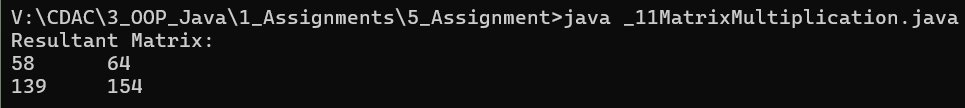
\includegraphics[width=0.8\textwidth]{11.png}
\end{center}

% 12

\section{}
\textbf{Task:} Write a C++ program to find the GCD of two numbers

\subsection{}
\begin{lstlisting}
#include <iostream>
using namespace std;
/**
 * Calculates the greatest common divisor (GCD) of two numbers.
 *
 * The GCD of two numbers is the largest number that divides both of them without leaving a remainder.
 *
 * This function uses the Euclidean algorithm to calculate the GCD.
 *
 * @param a The first number.
 * @param b The second number.
 * @return The greatest common divisor of a and b.
 */
int gcd(int a, int b) {
    // Base case: if b is 0, the GCD is a
    if (b == 0) return a;

    // Recursive case: calculate the GCD of b and a % b
    return gcd(b, a % b);
}

/**
 * The main function of the program.
 *
 * Reads two numbers from the user and prints the greatest common divisor of the two numbers.
 *
 * @return 0 if the program runs successfully.
 */
int main() {
    int a, b;
    // Read two numbers from the user
    cin >> a >> b;

    // Print the greatest common divisor of a and b
    cout << gcd(a, b) << endl;

    return 0;
}

\end{lstlisting}

\subsubsection{}
\begin{center}
    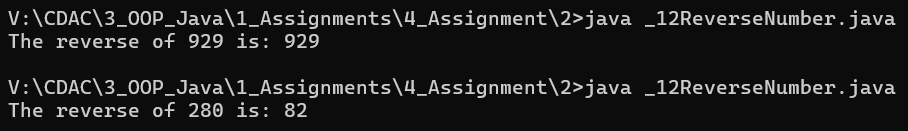
\includegraphics[width=0.8\textwidth]{12.png}
\end{center}

% 13

\section{}
\textbf{Task:} Write a C++ program to multiply two matrices.

\subsection{}
\begin{lstlisting}
#include <iostream>
#include <cstdlib>   // for rand() and srand()
#include <ctime>     // for time()
using namespace std;

/**
 * Multiplies two matrices.
 *
 * @param m1 The first matrix.
 * @param m2 The second matrix.
 * @return The product of the two matrices.
 */
int** multiply_matrices(int** m1, int rows1, int cols1, int** m2, int rows2, int cols2) {
    if (cols1 != rows2) {
        throw invalid_argument("The number of columns in the first matrix must match the number of rows in the second matrix.");
    }

    // Allocate memory for result matrix
    int** result = new int*[rows1];
    for (int i = 0; i < rows1; i++) {
        result[i] = new int[cols2];
        for (int j = 0; j < cols2; j++) {
            result[i][j] = 0; // initialize to 0
        }
    }

    // Matrix multiplication
    for (int i = 0; i < rows1; i++) {
        for (int j = 0; j < cols2; j++) {
            for (int k = 0; k < cols1; k++) {
                result[i][j] += m1[i][k] * m2[k][j];
            }
        }
    }

    return result;
}

// Utility function to print a matrix
void print_matrix(int** matrix, int rows, int cols, const string& name) {
    cout << "\n" << name << " (" << rows << "x" << cols << "):\n";
    for (int i = 0; i < rows; i++) {
        for (int j = 0; j < cols; j++) {
            cout << matrix[i][j] << "\t";
        }
        cout << endl;
    }
}

int main() {
    srand(time(0)); // Seed random number generator

    int rows1, cols1, rows2, cols2;

    cout << "Enter number of rows and columns for the first matrix: ";
    cin >> rows1 >> cols1;

    cout << "Enter number of rows and columns for the second matrix: ";
    cin >> rows2 >> cols2;

    if (cols1 != rows2) {
        cout << "Matrix multiplication not possible! Columns of first must equal rows of second.\n";
        return 1;
    }

    // Allocate and fill first matrix with random values
    int** m1 = new int*[rows1];
    for (int i = 0; i < rows1; i++) {
        m1[i] = new int[cols1];
        for (int j = 0; j < cols1; j++) {
            m1[i][j] = rand() % 10; // random values between 0–9
        }
    }

    // Allocate and fill second matrix with random values
    int** m2 = new int*[rows2];
    for (int i = 0; i < rows2; i++) {
        m2[i] = new int[cols2];
        for (int j = 0; j < cols2; j++) {
            m2[i][j] = rand() % 10;
        }
    }

    // Display input matrices
    print_matrix(m1, rows1, cols1, "Matrix 1");
    print_matrix(m2, rows2, cols2, "Matrix 2");

    // Multiply matrices
    int** result = multiply_matrices(m1, rows1, cols1, m2, rows2, cols2);

    // Display result
    print_matrix(result, rows1, cols2, "Resultant Matrix (M1 x M2)");

    // Free allocated memory
    for (int i = 0; i < rows1; i++) delete[] m1[i];
    delete[] m1;

    for (int i = 0; i < rows2; i++) delete[] m2[i];
    delete[] m2;

    for (int i = 0; i < rows1; i++) delete[] result[i];
    delete[] result;

    return 0;
}

\end{lstlisting}

\subsubsection{}
\begin{center}
    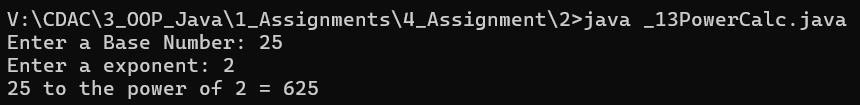
\includegraphics[width=0.8\textwidth]{13.png}
\end{center}

% 14

\section{}
\textbf{Task:} A number is an Armstrong number if the sum of its digits raised to the power of the number of digits is equal to the number itself (e.g., 153 = 1³ + 5³ + 3³).  Write a C++ program to check if a number is Armstrong.

\subsection{}
\begin{lstlisting}
#include <iostream>
#include <cmath>
using namespace std;

bool is_armstrong_number(int n) {
    int digits = 0;
    int original = n;
    int sum = 0;

    while (n > 0) {
        n /= 10;
        digits++;
    }

    n = original;
    while (n > 0) {
        int digit = n % 10;
        sum += pow(digit, digits);
        n /= 10;
    }

    return sum == original;
}

int main() {
    int n;
    cout << "Enter a number: ";
    cin >> n;

    if (is_armstrong_number(n)) {
        cout << n << " is an Armstrong number." << endl;
    } else {
        cout << n << " is not an Armstrong number." << endl;
    }

    return 0;
}
\end{lstlisting}

\subsubsection{}
\begin{center}
    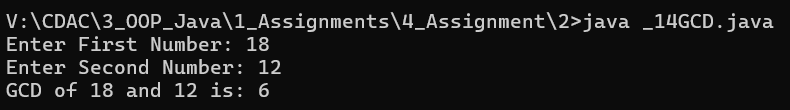
\includegraphics[width=0.8\textwidth]{14.png}
\end{center}

% 15

\section{}
\textbf{Task:} Write a C++ program to print Pascal’s triangle up to n rows.

\subsection{}
\begin{lstlisting}
#include <iostream>
using namespace std;

// Function to print Pascal's Triangle
void print_pascal_triangle(int n) {
    for (int i = 0; i < n; i++) {
        int value = 1; // First element of every row is 1
        
        // Print leading spaces for alignment
        for (int space = 0; space < n - i - 1; space++) {
            cout << "  ";
        }

        // Print values in the row
        for (int j = 0; j <= i; j++) {
            cout << value << "   ";
            value = value * (i - j) / (j + 1); // Compute next value in row
        }

        cout << endl;
    }
}

int main() {
    int n;
    cout << "Enter the number of rows: ";
    cin >> n;
    cout << "\nPascal's Triangle (" << n << " rows):\n";
    print_pascal_triangle(n);

    return 0;
}

\end{lstlisting}

\subsubsection{}
\begin{center}
    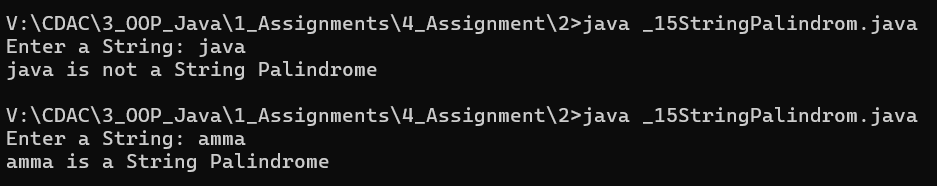
\includegraphics[width=0.8\textwidth]{15.png}
\end{center}


\end{document}



